\documentclass[11pt]{article}

% ---------------------------------------------------------------------------
% Structured Digital Ink as First-Class Model Context
% Research paper for the Neeh SDK.  Compile with: tectonic neeh-icf.tex
% ---------------------------------------------------------------------------

\usepackage[margin=1in]{geometry}
\usepackage{booktabs}
\usepackage{amsmath}
\usepackage{amssymb}
\usepackage{array}
\usepackage{multirow}
\usepackage{enumitem}
\usepackage{microtype}
\usepackage{xcolor}
\usepackage{titlesec}
\usepackage{caption}
\usepackage{listings}
\usepackage{pgfplots}
\pgfplotsset{compat=1.18}
\usetikzlibrary{arrows.meta,positioning,shapes.geometric}
\usepackage[htt]{hyphenat}
\usepackage[hidelinks]{hyperref}

% Let long monospace tokens (find_ink_moments, file paths) break instead of
% spilling into the margin, and give TeX a little slack as a last resort.
\emergencystretch=2em
\hyphenpenalty=1000
\tolerance=2000

\definecolor{neehblue}{HTML}{1d4ed8}
\definecolor{codebg}{HTML}{f4f5f7}
\definecolor{rulegray}{HTML}{888888}

\hypersetup{colorlinks=true, linkcolor=neehblue, citecolor=neehblue, urlcolor=neehblue}

\captionsetup{font=small, labelfont=bf}
\titleformat{\section}{\normalfont\Large\bfseries\color{black}}{\thesection}{0.6em}{}
\titleformat{\subsection}{\normalfont\large\bfseries}{\thesubsection}{0.6em}{}

\lstset{
  basicstyle=\ttfamily\small,
  backgroundcolor=\color{codebg},
  breaklines=true,
  frame=none,
  xleftmargin=1em,
  showstringspaces=false,
  columns=fullflexible,
}

\newcommand{\code}[1]{\texttt{#1}}
\newcommand{\tokens}[1]{\,{\small#1}}

\title{\vspace{-2.5em}\textbf{Structure Before Pixels: Deterministic Analysis and\\
Bounded Retrieval over Digital Ink as Model Context}}

\author{
  Kunwarbir Singh Padda\\
  \small Neeh SDK Project
}

\date{July 12, 2026}

\begin{document}
\maketitle

\begin{abstract}
\noindent
Digital ink --- handwriting, sketches, diagrams, and pen annotations --- is
almost always handed to software and to language-model agents as a rendered
image. That flattening is a \emph{many-to-one} map: two different stroke
histories can rasterize to byte-identical pixels while differing in draw order,
direction, pressure, and revision history, and once flattened none of that is
recoverable. This paper presents \textbf{Neeh}, a structured digital-ink SDK
that keeps ordered, timestamped, addressable strokes as the source of truth and
treats a raster as one derived, on-demand view among several. We describe the
system --- an immutable ink model, a compact model-facing \emph{Ink Context
Format} (ICF), deterministic geometric and temporal analyzers, query-aware
retrieval, a geometric structure recognizer, and a bounded
perception--action--feedback agent loop exposed over the Model Context Protocol
--- and we report two controlled experiments run through a fixed large model
(GPT-5.5 at high reasoning effort). In the first, \textbf{render-identical}
experiment, pairs of ink samples certified pixel-identical but differing on one
hidden history axis drive a raster-only model to \emph{exactly chance} accuracy
(0.50) while both structured facts and plain coordinate serialization recover
the answer perfectly (1.00); critically, the raster-only failure is
\emph{question-dependent} --- the model invents the same nonexistent visual cue
with full confidence on one task ($12/12$) yet honestly hedges on another
($12/12$) --- and adding structure to the \emph{same} image overrides the false
prior, grounding the answer in the actual coordinates or timestamps ($11$--$12/12$
vs $0/12$). In the
second, \textbf{token-budget} experiment, we show that model \emph{accuracy}
never degrades with ink density (perfect through 320 marks) but per-point and
per-mark serializations grow linearly and cross a representative context budget,
whereas an exact deterministic reducer answers the same question at
approximately constant ($\approx$270-token) cost. On the strength of this
evidence we argue --- against an initially attractive plan --- that a native
\emph{learned} ink encoder is not warranted: the accuracy gap such an encoder
would close does not exist at the densities tested, and the real problem is a
token-scaling problem that a deterministic analyzer solves exactly, without
training data, inference cost, or a new model artifact. The SDK is validated by
243 Python tests and two native (C++/C-ABI) suites, all passing. We close with
the empirical gate under which the learned-encoder question would be reopened.

\vspace{0.6em}
\noindent\textbf{Keywords:} digital ink; handwriting; stylus; model context;
language-model agents; deterministic analysis; Model Context Protocol; token
budget; representation; multimodal.
\end{abstract}

\section{Introduction}

Digital ink is a first-class input on tablets, styluses, and interactive
whiteboards, and it is increasingly something a language-model agent is asked to
read, reason about, and edit. The dominant way to feed ink to a model is to
render it: take a screenshot or export a PNG and attach it as an image. This is
simple, it composes with any vision-language model, and it is lossy in a
specific, consequential way.

A rendered image is a \emph{many-to-one} function of the underlying ink. Let
$I$ be an ink document --- an ordered set of strokes, each an ordered sequence
of timestamped points with pressure and tilt --- and let $R(\cdot)$ be the
rasterizer. Two documents $I_1 \neq I_2$ that differ only in the \emph{order}
their strokes were drawn, the \emph{direction} a stroke was traced, the
\emph{pressure} applied, or whether some ink was later crossed out and replaced,
can satisfy $R(I_1) = R(I_2)$ exactly. The pixels are identical; the histories
are not. Once an agent sees only $R(I)$, the distinguishing information is not
merely hard to recover --- it is provably absent.

This matters because a large and useful class of questions about ink depends on
exactly that discarded information: \emph{Which shape was drawn first?} \emph{In
which direction was this stroke traced?} \emph{Was this figure crossed out and
replaced, or is it the current answer?} \emph{What changed since I last looked?}
A raster cannot answer any of these, and --- as we show in
Section~\ref{sec:results} --- a capable model given only a raster does not
reliably say ``I cannot tell.'' It produces a fluent, confident, and false
justification.

\paragraph{Thesis.} Neeh inverts the usual pipeline. Instead of starting from an
image and layering recognition on top, it keeps the ink's native structure ---
ordered, timestamped, addressable strokes --- as the canonical representation,
and renders an image as one \emph{output} of that structure, fetched on demand
only when pixels answer better than structure does (chiefly for reading
handwritten content). Around this it places deterministic local computation:
mechanical questions about time and geometry are answered \emph{exactly and
locally}, and the model receives a small, typed conclusion plus recoverable
evidence rather than a serialized page to search.

This is not a claim of novelty for ``structure over pixels'' in general: the same
trade-off is well established in web and computer-use agents, which converged on
sending a structured accessibility tree by default and a screenshot only as a
fallback~\cite{setofmark,omniparser,memgpt}. Neeh's contribution is to work out
what the analogous structured representation should be \emph{for digital ink},
where no such standard shape existed, and to measure whether it earns its place
against both the raster baseline and the more ambitious alternative of a learned
ink encoder.

\paragraph{Contributions.}
\begin{enumerate}[leftmargin=1.4em, itemsep=2pt]
\item \textbf{A structured ink SDK} (\S\ref{sec:system}): an immutable
  ink/document/canvas model with stable stroke IDs, timing, pressure, tilt, and
  authorship; a compact model-facing \emph{Ink Context Format v1}; deterministic
  analyzers; query-aware temporal retrieval; a geometric structure recognizer;
  and a bounded agent loop over the Model Context Protocol, with a C++17 core and
  versioned C ABI.
\item \textbf{A render-identical experiment} (\S\ref{sec:move1}) that isolates
  the unique value of ink structure from general model quality by holding the
  pixels byte-constant. It shows a raster-only model pinned at chance and, more
  importantly, that its failure mode is \emph{question-dependent}: it confabulates
  a nonexistent visual cue with full confidence on one task ($12/12$) yet honestly
  hedges on another ($12/12$), and supplying structure over the same image
  \emph{overrides} the false prior --- a product-safety result independent of any
  representation-learning question.
\item \textbf{A token-budget experiment} (\S\ref{sec:move1b}) that separates two
  things usually conflated: reasoning \emph{accuracy} (which does not degrade
  with ink density) and \emph{context cost} (which does, linearly, for
  serialized ink). It shows an exact deterministic reducer holding a temporal
  task at approximately constant cost where serialization crosses budget.
\item \textbf{A negative architectural result} (\S\ref{sec:discussion}): on the
  evidence gathered, a native learned ink encoder is not warranted, together
  with an explicit, falsifiable gate for reopening that decision.
\end{enumerate}

All model calls in this work go through a fixed configuration --- GPT-5.5 at high
reasoning effort, invoked through a command-line login rather than a raw API ---
and every experiment is run from certified-balanced, synthetic ink so that a
raster-only floor is provably chance by construction. We are explicit about the
limits of that design in Section~\ref{sec:threats}.

\section{Background and Related Work}
\label{sec:related}

\subsection{Representing ink for recognition}
The closest body of work treats digital ink as an input to \emph{handwriting
recognition}. Fadeeva et al.~\cite{fadeeva2024} show that off-the-shelf
vision-language models can consume online handwriting as a combination of a
rendered image and a serialized stroke-as-text sequence with \emph{no
architecture change}, matching specialized recognizers. Col-OLHTR~\cite{cololhtr}
trains multimodally on trajectory and image but infers from the trajectory alone
via an alignment module. Lodh et al.~\cite{lodh2025} fuse online $(x,y,\text{pen})$
signals and offline image features in a shared latent space through learnable
queries. ScribeTokens~\cite{scribetokens} defines a fixed-vocabulary ink
tokenization with next-ink-token pretraining, achieving strong character error
rates --- but with a small from-scratch transformer, on handwriting \emph{text},
not diagrams or reasoning. InkSight~\cite{inksight} derenders offline photographs
of handwriting into online ink by teaching a VLM to ``read and write.''

Two things are true of this literature taken together. First, it establishes ---
as an existence proof --- that some representation beyond a PNG carries the
ink-specific signal, since serialized strokes already recover recognition
performance. Second, \emph{every} ink-specific result is handwriting-text
recognition or generation; none connects an ink encoder to a frozen large model
for \emph{reasoning} over temporal, spatial, and revision structure. A single
data point from ScribeTokens is worth isolating: randomly-initialized ink tokens
are ignored (attention near chance) until self-supervised next-ink-token
pretraining forces the model to attend to them --- and a \emph{frozen} model
cannot run that pretraining on itself, so the cold-start problem for a frozen
ink bridge is strictly harder than the recognition literature makes it look.

\subsection{Frozen-model bridges}
The idea of bridging a new modality into a frozen language model with a small
learned adapter is well established: Flamingo~\cite{flamingo} interleaves
vision and text through gated cross-attention; BLIP-2~\cite{blip2} inserts a
lightweight querying transformer (Q-Former) between a frozen image encoder and a
frozen LLM; LLaVA~\cite{llava} projects visual features into the language
embedding space with instruction tuning. These precedents make a learned
ink$\rightarrow$model bridge \emph{plausible}, and an early plan for Neeh
proposed exactly that as a research track. This paper's evidence is what led us
not to build it (\S\ref{sec:discussion}).

\subsection{Structure over pixels in agents}
Outside ink, the strongest analogy is the recent convergence of GUI and web
agents on structured context. Set-of-Mark prompting~\cite{setofmark} overlays
labeled marks so a model can reference elements by ID rather than pixel
coordinates; OmniParser~\cite{omniparser} converts a UI screenshot into a
structured, addressable element list; MemGPT~\cite{memgpt} pages bounded context
in and out rather than sending everything. Microsoft's Playwright automation
tooling follows the identical shape --- an accessibility snapshot by default, a
vision screenshot only as a fallback for elements the tree does not cover ---
with the explicit finding that an ID-grounded action on a well-represented
element is \emph{more reliable}, not merely cheaper, than a vision-grounded one.
Neeh is a deliberate transposition of that pattern to digital ink, where the
``accessibility tree'' equivalent had no established form.

\subsection{Diagrams as code}
A parallel line reasons over diagrams by first recovering a symbolic program:
Draw-with-Thought, SketchAgent, and CoMT~\cite{diagramcode} operate on
code or XML representations of a figure rather than on raw sensor ink with
timing, pressure, and revision history. This is the correct competitive
baseline for any structured-ink claim, and it is notably the \emph{same shape}
as what Neeh already ships: a geometric recognizer plus a structured index plus
tool calls \emph{is} a ``recognize $\rightarrow$ structured text $\rightarrow$
model'' pipeline. Neeh's structured path is therefore not competing with a weak
baseline; it is an instance of the strong one, specialized to ink and augmented
with the temporal and revision signals diagram-as-code discards.

\subsection{Interchange and protocol}
For persistence, Neeh maps to the Universal Ink Model (UIM)~\cite{uim}, an
open ink interchange standard, through a versioned profile. Established
ink-markup standards --- UIM and W3C InkML~\cite{inkml} --- are full-fidelity
\emph{interchange} formats, and ICF is deliberately not one: it is a bounded,
lossy-by-choice \emph{model-facing} snapshot (\S\ref{sec:system}) that a producer
may simplify to fit a token budget, which an interchange format must never do.
For agent integration Neeh exposes its perception surface over the Model Context
Protocol~\cite{mcp}, so that read-only perception runs as an external process
that cannot mutate the live document.

\section{System Architecture}
\label{sec:system}

Neeh is organized as one path from captured strokes to a validated edit. Each
stage is a distinct module; a raster is a derived, lossy view produced from the
structure at any stage, never upstream of it. Table~\ref{tab:stages} lists the
stages.

\begin{table}[t]
\centering
\small
\begin{tabular}{@{}>{\raggedright\arraybackslash}p{0.22\linewidth} >{\raggedright\arraybackslash}p{0.46\linewidth} >{\raggedright\arraybackslash}p{0.24\linewidth}@{}}
\toprule
\textbf{Stage} & \textbf{What it is} & \textbf{Module} \\
\midrule
Raw ink & Ordered, timestamped points with pressure/tilt; strokes; pages/layers & \code{neeh.ink}, \code{neeh.document} \\
Rendered image & SVG, optional PNG, token-cheap ASCII views of a page or region & \code{neeh.rendering} \\
Recognition & Geometric clustering and directed links between marks (shape recognition, not transcription) & \code{neeh.semantics} \\
Deterministic analysis & Exact local answers to temporal/geometric questions, bounded regardless of page size & \code{neeh.agents.analyzers} \\
Temporal structure & Ink grouped into creation ``moments,'' ranked and retrievable by relevance & \code{neeh.agents.timeline} \\
Structured context & Compact, addressable model-facing snapshots (ICF, ink-index) & \code{neeh.context} \\
Agent tools & Bounded mutation API and read-only perception surface & \code{neeh.tools}, \code{neeh.agents.iai} \\
\bottomrule
\end{tabular}
\caption{Neeh's modules correspond to points on one path from raw ink to an
applied edit. The inversion at the center of the project: existing pipelines
start from an image and add recognition; Neeh starts from structure and renders
an image as one output of it.}
\label{tab:stages}
\end{table}

\subsection{Ink model and document}
The canonical representation is immutable. A \code{Point} carries $x, y$, a
timestamp $t_{ms}$, pressure, and tilt. A \code{Stroke} is an ordered tuple of
points with a style, an author, a creation time, and a \emph{stable ID}. Strokes
live in ordered \code{Layer}s inside \code{Page}s inside a \code{Document}. The
document is the single source of truth; every representation sent to a model is
derived from it on demand and none is itself where state lives. This lets Neeh
change what it shows a model without ever touching what it stores. A
\code{Canvas} session wraps a document with selection, atomic edits, and
undo/redo.

\subsection{The Ink Context Format (ICF v1)}
ICF is a bounded, model-facing snapshot of one page (protocol identifier
\code{ink-context/v1}). It is not a persistence format. A payload is a JSON
object with a fixed envelope: a \code{page} record (id, size, background), a
\code{raster} record describing an \emph{optional} attached image, an \code{ink}
record, and a \code{semantics} array. The \code{ink} record encodes stroke
geometry as compact SVG paths on an integer grid, in document draw order, with
each path keyed by its stable stroke ID:

\begin{lstlisting}
<path id="st_..." d="M18 18l4 1 3 -2"/>
\end{lstlisting}

A crucial separation of concerns runs through the format: the SVG grid is a
compact \emph{display} coordinate system, but any coordinate a consumer may pass
back to a tool call --- regions, bounding boxes, semantic anchors --- must be in
\emph{page units}. Producers may resample or simplify a stroke (e.g. by
Ramer--Douglas--Peucker simplification) to meet a character budget, declaring the
operating point in a \code{rate\_point} field, but simplification must never
change a stroke's ID or its order. Figure~\ref{fig:icf} shows a complete payload
emitted by the SDK for a two-stroke page, in which the two coordinate systems are
visible side by side: the \code{svg} paths live on a $181\times256$ grid, while
the \code{bboxes} that a tool call would consume are in page units. The design
rationale, and the decision to make the structured index (not the raster) the
default channel, is recorded as Architecture Decision Record (ADR)
0001~\cite{adr1}.

\begin{figure}[t]
\begin{lstlisting}
{
  "schema": "ink-context/v1",
  "page": { "id": "pg_1efb63c8", "width": 1000, "height": 1414,
            "background": "#ffffff" },
  "raster": { "format": "png", "transport": "none",
              "coordinate_space": "page", "region": null },
  "ink": {
    "encoding": "svg-paths/grid", "grid": [181, 256],
    "drawn_order": true, "region": null,
    "stroke_count": 2, "included_stroke_count": 2,
    "omitted_older_stroke_count": 0, "truncated": false,
    "svg": "<svg viewBox=\"0 0 181 256\">
      <path id=\"st_9e170117\" d=\"M22 25l3 -2 3 -3 3 -2 ...\"/>
      <path id=\"st_768e944d\" d=\"M22 33l4 0 4 0 4 0 ...\"/></svg>",
    "bboxes": { "st_9e170117": [120, 90, 240, 140],
                "st_768e944d": [120, 180, 240, 180] }
  },
  "semantics": []
}
\end{lstlisting}
\vspace{-0.4em}
\caption{A complete \code{ink-context/v1} payload produced by the SDK for a
two-stroke page (a caret over an underline). Stroke IDs are abbreviated and long
\code{d} attributes truncated for space. Note the deliberate two-coordinate-system
design: \code{svg} geometry is on the compact integer \code{grid}, but every
\code{bbox} --- the only coordinates a consumer passes back to a tool --- is in
page units.}
\label{fig:icf}
\end{figure}

\subsection{Deterministic analyzers (ink-analysis v1)}
The analysis plane answers mechanical questions by \emph{computing} the exact
answer locally rather than asking a model to search a serialized page. The
principle: do not spend model context on a fact Neeh can calculate. An analyzer
reads the complete local document but returns only task-relevant, typed
evidence, so prompt cardinality is bounded by the \emph{operation}, not the page
stroke count. The shipped operations are \code{latest\_mark} (the most recently
drawn visible stroke, with time, bbox, center, page half, direction, duration,
and pressure summary), \code{creation\_order} (bounded chronological order of
explicitly named strokes), \code{stroke\_dynamics} (direction/duration/pressure
for named strokes), and \code{cross\_out\_candidates} (timeline episodes whose
geometry suggests a later stroke passes through older ink --- returned as
hypotheses, never asserted as user intent). Every response is stamped
\code{deterministic=true} with source and matched stroke counts. The measured
cost consequence of this design is the subject of \S\ref{sec:move1b}.

\subsection{Temporal structure and retrieval}
The timeline plane (\code{ink-timeline/v1}) groups ink into creation episodes
(``moments'') and ranks them by relevance to a query, so an agent can retrieve
only the moments and regions that matter instead of receiving the whole page.
This is the ``promote only relevant evidence into a working set'' stage.

\subsection{Geometric structure recognizer}
\code{neeh.semantics} is a deterministic, geometry-based recognizer that turns
strokes into clusters and directed links: it identifies long straight strokes as
connectors, small bent strokes riding a connector endpoint as arrowheads, groups
the remainder by bounding-box union-find, and binds each connector's endpoints to
the nearest clusters --- taking link direction from the arrowhead when present,
else from draw order at lower confidence. Every output is a valid ICF
\code{semantics} entry with page-unit coordinates, resolvable stroke IDs, a
\code{confidence}, and a \code{source} tag, so recognizer \emph{claims} are never
conflated with exact \emph{measurements}. Recognition here is shape structure,
deliberately not handwriting transcription, which remains a raster-on-demand
task.

\subsection{The Ink Agent Interface: a bounded loop}
The agent layer (\code{neeh.agents.iai}) implements a
perception--action--feedback loop that is bounded at every stage:

\begin{enumerate}[leftmargin=1.4em, itemsep=1pt]
\item \textbf{Bootstrap.} A budgeted \code{page\_map}, the ink new since the
  model's last turn, and (for policies that allow it) a set of typed read-only
  perception actions with their remaining budget.
\item \textbf{Perceive, if needed.} The model may call \code{find\_marks},
  \code{analyze\_ink}, \code{view\_region}, \code{find\_ink\_moments},
  \code{inspect\_ink\_moment}, \code{get\_ink}, or \code{expand\_relations} ---
  each bounded, each declaring the page-space region or fidelity it covers,
  exposed over a read-only stdio MCP server so perception cannot mutate the live
  document.
\item \textbf{Plan.} The model returns a batch of edit-tool calls.
\item \textbf{Validate.} The batch is replayed atomically on a document clone.
\item \textbf{Repair, once.} A failing batch gets exactly one corrected attempt
  with the validation feedback attached; there is no open-ended retry loop.
\item \textbf{Apply.} Only a fully valid batch touches the live document.
\end{enumerate}

Figure~\ref{fig:loop} shows the loop. Perception is read-only and bounded; only
a batch that survives atomic validation on a clone --- with at most one repair
pass --- is ever applied to the live document.

\begin{figure}[t]
\centering
\resizebox{\linewidth}{!}{%
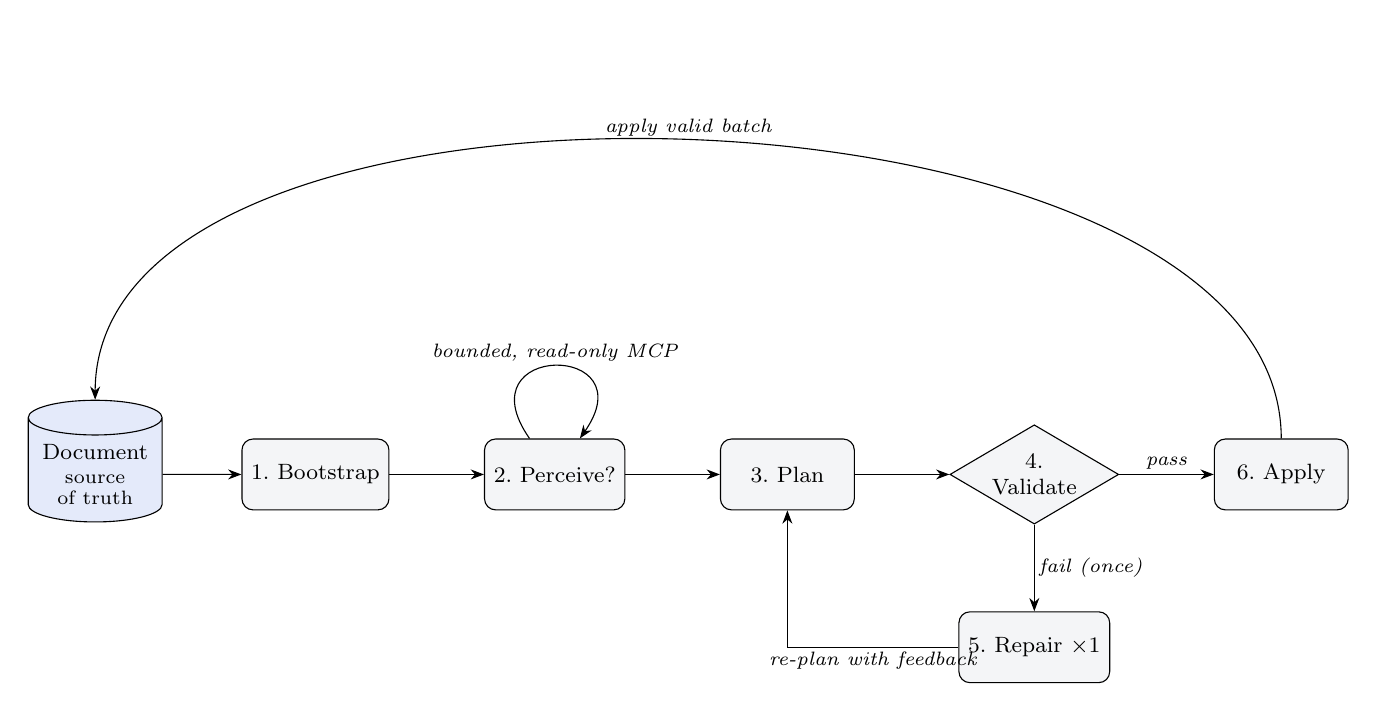
\begin{tikzpicture}[
  >=Stealth, font=\footnotesize,
  stage/.style={draw, rounded corners, minimum height=9mm, minimum width=17mm,
    align=center, fill=codebg},
  doc/.style={draw, cylinder, shape border rotate=90, aspect=0.28,
    minimum height=13mm, minimum width=17mm, align=center, fill=neehblue!12},
  dec/.style={draw, diamond, aspect=1.7, inner sep=1pt, align=center, fill=codebg},
  lbl/.style={font=\scriptsize\itshape, inner sep=1.5pt},
]
\node[doc] (d) {Document\\[-1pt]\scriptsize source\\[-2pt]\scriptsize of truth};
\node[stage, right=10mm of d]  (b)  {1.~Bootstrap};
\node[stage, right=12mm of b]  (p)  {2.~Perceive?};
\node[stage, right=12mm of p]  (pl) {3.~Plan};
\node[dec,   right=12mm of pl] (v)  {4.\\Validate};
\node[stage, right=12mm of v]  (a)  {6.~Apply};
\node[stage, below=11mm of v]  (r)  {5.~Repair $\times 1$};

\draw[->] (d) -- (b);
\draw[->] (b) -- (p);
\draw[->] (p) -- (pl);
\draw[->] (pl) -- (v);
\draw[->] (v) -- node[lbl, above]{pass} (a);
\draw[->] (v) -- node[lbl, right]{fail (once)} (r);
\draw[->] (r) -| node[lbl, below, pos=0.25]{re-plan with feedback} (pl);
\draw[->] (p) to[out=125,in=55,looseness=6]
  node[lbl, above]{bounded, read-only MCP} (p);
\draw[->] (a) to[out=90,in=90, looseness=0.8]
  node[lbl, above]{apply valid batch} (d);
\end{tikzpicture}%
}
\caption{The bounded perception--action--feedback loop
(\S\ref{sec:system}). The document is the single source of truth; a budgeted
bootstrap and optional read-only perception feed a planned batch of edits, which
is validated atomically on a clone. A failing batch earns exactly one repair
pass; only a fully valid batch is applied back to the live document. Every stage
carries a fixed budget, so cost stays predictable as the page grows.}
\label{fig:loop}
\end{figure}

The loop has a fixed action budget, a fixed observation-character budget, a
fixed raster-pixel budget, and exactly one repair pass, so context cost and
reasoning cost stay predictable as a page grows rather than scaling with page
size or trajectory length. Model turns are \emph{stateless and ephemeral};
continuity comes from Neeh recomputing what changed from the document's own
timestamps, not from provider-side conversation memory --- a decision measured
and recorded as ADR 0003~\cite{adr3}.

\subsection{Native core}
The ink/document substrate and SVG/RGBA rendering are also implemented in a
C++17 core behind ABI version~1 of a C interface, so native hosts can consume the
same primitives; a CMake package exports a \code{Neeh::Core} target. The native
suites are part of the validation reported in \S\ref{sec:software}.

\section{Experimental Methodology}
\label{sec:method}

\subsection{Model access and configuration}
Every model call is issued to \textbf{GPT-5.5 at high reasoning effort},
invoked through the model provider's command-line login (Codex CLI) rather than
a raw API, and hard-pinned to that model and effort in the harness. Fixing a
single strong model and configuration is deliberate: the experiments are designed
to isolate the effect of the \emph{input representation}, so the model is held
constant and only the representation varies. Responses are constrained to a JSON
answer schema (\code{\{answer, why\}}) so that both the choice and its stated
justification are captured for every trial.

Critically, every condition --- including the raster-only arm --- receives an
\emph{identical} preamble stating the coordinate convention and that a stroke's
points are listed in the order the pen drew them; only the perception payload
(an image, a structured record, or a coordinate stream) differs between
conditions. The raster arm is therefore not handicapped by weaker instructions:
it is told the same facts could matter and still cannot answer, because the
pixels genuinely lack the signal. This forecloses a ``the structured prompt was
primed'' reading of the gap.

\subsection{Token estimation}
Because the two headline experiments turn on cost as well as accuracy, we use a
single deterministic token estimate throughout: characters$/4$ for text, plus
image pixels$/750$ for any attached raster (cropped to the ink's bounding box).
This estimate is computable without any model call, which is what makes the
token-scaling curves in \S\ref{sec:move1b} reproducible offline.

\subsection{Experiment 1 --- Render-identical pairs}
\label{sec:m1method}
To separate the unique value of ink structure from general model competence, we
construct pairs of ink samples that are \textbf{certified byte-identical in
pixels} yet differ on exactly one hidden axis of ink history. The generator
supports three such render-identical axes --- direction, creation order, and pen
pressure (all certify pixel-identical: $18/18$ pairs under \code{-{}-dry-run}) ---
and we report the two whose hidden signal is a \emph{temporal/ordinal} property of
the draw history, the canonical case for ``pixels destroy ink history.'' Pen
pressure is also render-identical (the renderer ignores it), but its answer is a
literal per-point field value rather than a fact inferred from the stroke
sequence, so we set it aside. The two reported axes are:

\begin{itemize}[leftmargin=1.4em, itemsep=1pt]
\item \textbf{direction}: one horizontal stroke, drawn left-to-right in one twin
  and right-to-left in the other. Because a rasterizer that ignores draw
  direction and pressure produces the same image either way, \emph{both twins are
  rendered from a single shared canonical page}, guaranteeing byte identity.
\item \textbf{order}: a rectangle and an arrow, with the creation timestamps
  swapped between twins. The strokes are stored in a \emph{fixed spatial order}
  (box then arrow) so list position never leaks the answer; only the creation
  time distinguishes them.
\end{itemize}

Each twin is posed the same forced-choice question, whose answer lives only in
the hidden history, and is run through the same model under three input
conditions:
\begin{itemize}[leftmargin=1.4em, itemsep=1pt]
\item \textbf{png}: the cropped page raster only --- the theoretical floor, since
  the information is provably absent.
\item \textbf{png+struct}: the raster plus a structured ink record (shape label,
  creation time, and a subsampled $(x,y,t,\text{pressure})$ stream) --- the
  Neeh ``recognizer index'' ceiling.
\item \textbf{coords}: a plain coordinate serialization, no image --- a
  Fadeeva-style~\cite{fadeeva2024} textual encoding.
\end{itemize}

A guard certifies that every pair rasterizes to identical decoded RGB pixels
before any model call; a failed certification would mean a generator leaked
signal into the image and invalidates that pair. The reported sweep certified
\textbf{12 of 12 pairs} identical (6 per axis). Twins carry opposite ground-truth
answers, so a model that cannot see the hidden axis and defaults to one option is
\emph{exactly} at chance by construction. The sweep issues
\textbf{72 model calls} (2 axes $\times$ 3 conditions $\times$ 12 trials).

\subsection{Experiment 2 --- Token-budget scaling}
\label{sec:m1bmethod}
The second experiment asks what happens as ink density grows. On a page of $N$
marks --- each mark a single stroke, so mark count equals stroke count --- drawn
at distinct times, the task is temporal and needs the whole
page: identify the mark drawn \emph{last} and report whether its center lies in
the upper or lower half. The last-drawn mark is forced into the target half so
the dataset stays balanced (a raster, having no timestamps, is at chance). We
sweep $N \in \{4, 16, 48, 128, 320\}$ with 6 trials per size, comparing four
representations:
\begin{itemize}[leftmargin=1.4em, itemsep=1pt]
\item \textbf{png}: dense raster only --- floor (no timing).
\item \textbf{coords-full}: every mark's $(x,y,t,\text{pressure})$ stream --- grows
  $\sim$linearly with $N$.
\item \textbf{index-compact}: every mark as \code{\{i, created\_at\_ms, center\}}
  --- also linear, smaller constant.
\item \textbf{analyzer-reduced}: the output of Neeh's exact \code{latest\_mark}
  reducer --- bounded, $O(1)$ evidence regardless of $N$.
\end{itemize}
The token-versus-$N$ curves are deterministic and need no model calls; a live
sweep additionally measures whether accuracy degrades as the relevant timestamp
is buried among $N$ distractors. To be precise about what is measured versus
computed: the live accuracy sweep covers the two \emph{serialized} structured
arms (\code{coords-full}, \code{index-compact}), whose accuracy \emph{and} token
cost are both reported from the run. The \code{png} and \code{analyzer-reduced}
token costs are deterministic estimates, not live accuracy runs, and for good
reason: \code{png} cannot answer a timing question at all (its accuracy is the
chance floor by construction), and the analyzer's single-record output is
\emph{exact} by construction --- it is separately unit-tested to reduce a
320-stroke page to one constant-size record (\S\ref{sec:software}) --- so pricing
it, rather than re-deriving a trivially-correct model answer over one typed fact,
is the honest comparison. The live sweep therefore issues \textbf{60 model calls}
(5 sizes $\times$ 2 serialized arms $\times$ 6 trials).

\subsection{Supporting measurements}
Three further internal experiments, recorded in the project's ADR log, inform the
architecture and are summarized in \S\ref{sec:support}: a context-arm comparison
on real ink~\cite{adr1}; a delta-context and session-transport study~\cite{adr3};
and a two-case controlled-pair perception smoke test.

\section{Results}
\label{sec:results}

\subsection{Experiment 1: structure recovers what pixels cannot, and pixels confabulate}
\label{sec:move1}

Table~\ref{tab:move1} gives the outcome. On both airtight axes the raster-only
condition sits at \textbf{exactly chance} (0.50), while both structured
conditions reach \textbf{perfect} accuracy (1.00). The result is not marginal:
the model answered the first option on every raster-only direction trial, so the
0.50 is a mechanical default over balanced twins, not noisy guessing. Under a
one-sided binomial test against the $0.5$ chance rate, the structured arms'
$12/12$ is significant at $p = 2^{-12} \approx 2.4\times10^{-4}$ per cell, while
the raster-only $6/12$ is exactly the chance expectation ($p = 0.61$).

\begin{table}[t]
\centering
\small
\begin{tabular}{@{}l l ccc@{}}
\toprule
\textbf{Axis} & \textbf{Metric} & \textbf{png} & \textbf{png+struct} & \textbf{coords} \\
\midrule
\multirow{2}{*}{direction}
 & accuracy & 0.50 & \textbf{1.00} & \textbf{1.00} \\
 & mean tokens & 242 & 327 & \textbf{221} \\
\midrule
\multirow{2}{*}{order}
 & accuracy & 0.50 & \textbf{1.00} & \textbf{1.00} \\
 & mean tokens & 686 & 877 & \textbf{232} \\
\bottomrule
\end{tabular}
\caption{Render-identical experiment (GPT-5.5, high reasoning effort; $n=12$
trials per cell; 12/12 pairs certified pixel-identical). The raster-only floor is
exactly chance; structure recovers the answer perfectly; plain coordinate
serialization does so at the \emph{lowest} token cost of the three.}
\label{tab:move1}
\end{table}

Three findings follow.

\paragraph{(1) The PNG floor is chance, and it is mechanical.} The information is
provably absent from the pixels, and the model's balanced-twin accuracy of 0.50
confirms it empirically.

\paragraph{(2) Structure recovers it perfectly, with real inference.} Both
structured conditions reach 1.00 and cite exact evidence. A representative
\code{coords} justification: \emph{``the stroke points are ordered from $x=160$
at the left end to $x=786.7$ at the right end, so it was drawn left-to-right.''}
This is grounded reasoning over the recovered signal, not a lucky guess, and it is
the exact mirror of finding~(3): where the raster arm grounds $0/12$ of its
answers in a checkable fact, the structured arms ground essentially all of theirs
in the actual data. Coding each justification for whether it cites a specific
coordinate (direction) or creation timestamp (order), \code{png+struct} does so
in $12/12$ trials on both axes and \code{coords} in $11$--$12/12$, against
$0/12$ for the raster arm, which cites invented visual cues instead. Structure
does not merely raise the score; it changes the \emph{kind} of answer from an
unfalsifiable assertion to a verifiable one. Notably, \code{coords} is not only
tied for best accuracy but is the
\emph{cheapest} channel --- 221 tokens on direction and 232 on order, roughly a
third of \code{png+struct} on the order axis --- because it sends the point
stream without also paying for an image.

A second, subtler asymmetry hides in the same token columns. Both axes pose a
one-bit question over roughly two strokes, yet the raster cost nearly triples
between them --- 242 tokens on direction versus 686 on order ($2.8\times$) ---
simply because the rectangle-and-arrow scene inks more of the page than a single
horizontal stroke. The coordinate cost, by contrast, is essentially flat across
the two ($221$ vs $232$, $1.05\times$). Raster cost is metered by \emph{inked
area}, not by the information a task actually needs; structured cost tracks the
ink's complexity. This is the same property that makes the raster a bounded but
task-blind channel in Experiment~2, seen here from the cost side.

\paragraph{(3) The failure mode is confabulation, not honest uncertainty.} This
is the most consequential finding. On the direction axis, the raster-only model
did not abstain; it \emph{invented} pixel evidence that cannot exist:
\emph{``the right endpoint appears slightly tapered and lighter like a pen lift,
while the left endpoint looks more blunt like the initial contact.''} There is no
taper --- both ends are identical round caps and the renderer ignores pressure
entirely. What makes this more than a one-off slip is its \emph{systematicity}:
across all $12/12$ direction trials the model invents the \emph{same} nonexistent
cue --- a tapered or lifted right endpoint --- concludes the pen finished on the
right, and therefore answers ``left-to-right'' on every twin ($12/12$). It is a
fixed, reproducible hallucinated prior, not random error, and it is precisely
what pins the raster arm to chance: identical answers on twins that carry
opposite ground truth.

Crucially, this failure is \emph{not uniform} --- it is triggered by the question,
which is a more precise and more actionable result than ``raster models
confabulate.'' The two axes split perfectly. On direction, $12/12$ justifications
fabricate the nonexistent tapered endpoint and $0/12$ hedge. On order --- ``which
of these two shapes was drawn first?'' --- the split inverts: $0/12$ fabricate and
$12/12$ openly admit the guess (\emph{``with no ink history available, stroke
order cannot be determined from the image alone, so this is only a visual best
guess''}). Both conditions are forced to pick one of two options --- the answer
schema offers no ``unknown,'' so neither can formally abstain --- yet the
free-text justification still separates honesty from fabrication cleanly. The
model confabulates confidently \emph{exactly where it holds a plausible-but-false
visual prior} (endpoint shape implies stroke direction) and correctly signals
uncertainty where no such prior exists (two disjoint shapes carry no visual order
cue). The dangerous case is therefore not ``the raster always lies'' but ``the
raster lies confidently precisely where a false prior makes the lie feel
grounded'' --- the harder failure to catch. And the cure is directly observable:
the \code{png+struct} arm sees the \emph{same image} plus the structured record,
and adding structure flips the model completely --- from $12/12$ invoking the
false taper prior and $0/12$ grounded (\code{png}) to $0/12$ taper and $12/12$
grounded in the actual coordinates (\code{png+struct}). With the pixels held
constant, structure does not merely add a channel the model averages in; it
\emph{overrides} the false visual prior, and the fabrication vanishes.
Table~\ref{tab:coding} tabulates the full justification coding behind findings~(2)
and~(3). Shipping structured ink context is therefore a \emph{safety} argument by
itself, independent of any efficiency or representation-learning question: it
removes the false prior's opening by supplying the actual draw history, converting
a confident fabrication into a grounded, checkable answer.

\begin{table}[t]
\centering
\small
\begin{tabular}{@{}ll c ccc@{}}
\toprule
\textbf{Axis} & \textbf{Condition} & \textbf{Acc.} & \textbf{Fabricates} & \textbf{Hedges} & \textbf{Grounds} \\
 & & & \footnotesize false cue & \footnotesize admits guess & \footnotesize in exact data \\
\midrule
\multirow{3}{*}{direction}
 & \code{png}        & 0.50 & \textbf{12/12} & 0/12 & 0/12 \\
 & \code{png+struct} & 1.00 & 0/12 & 0/12 & \textbf{12/12} \\
 & \code{coords}     & 1.00 & 0/12 & 0/12 & \textbf{11/12} \\
\midrule
\multirow{3}{*}{order}
 & \code{png}        & 0.50 & 0/12 & \textbf{12/12} & 0/12 \\
 & \code{png+struct} & 1.00 & 0/12 & 0/12 & \textbf{12/12} \\
 & \code{coords}     & 1.00 & 0/12 & 0/12 & \textbf{12/12} \\
\bottomrule
\end{tabular}
\caption{Justification coding for Experiment~1 ($n=12$ per cell). Each trial's
free-text rationale is classified as fabricating a nonexistent visual cue,
honestly hedging (admitting the answer cannot be determined from the image), or
grounding in an exact coordinate or timestamp. The raster-only failure is
\emph{question-dependent} --- fabrication on direction, honest hedging on order ---
and adding structure to the \emph{same} image (\code{png+struct}) replaces both
with grounded reasoning.}
\label{tab:coding}
\end{table}

\paragraph{What the experiment does and does not claim.} The bare
$0.50\rightarrow1.00$ accuracy gap is \emph{expected by construction}: we
engineered the pixels to lack the answer, so a raster model must be at chance and
a structure-aware one can be perfect. That gap is the experiment's premise, not
its finding. Two results, by contrast, are \emph{not} entailed by the
information-theoretic setup and are the actual contribution: the behavioral split
above (fabrication versus honest hedging is question-dependent, which information
theory alone does not predict), and the cost result --- structure is strictly
\emph{cheaper} than the raster it beats (Table~\ref{tab:move1}), and cheaper still
than the analyzer makes it (\S\ref{sec:move1b}). Neither followed from the pixels
lacking the bits.

\subsection{Experiment 2: accuracy is invariant to density; only cost scales}
\label{sec:move1b}

The second experiment cleanly separates two properties usually conflated.

\paragraph{Accuracy does not degrade with density.} Both \code{coords-full} and
\code{index-compact} held \textbf{1.00 accuracy at every density} from $N=4$
through $N=320$ (6/6 trials per cell). The relevant timestamp did not become hard
to find as distractors multiplied; the model's \emph{reasoning} never broke down.
The justifications show \emph{why}: the grounding does not decay with density.
Coding all 60 trials, the model cites a specific center-$y$ in $60/60$ and the
exact latest \code{created\_at\_ms} in $58/60$ --- and at the hardest setting,
$N=320$ with 320 distractors, it still does both in $12/12$. It is not guessing
its way to $1.00$; it is reading the correct field exactly, even buried. This is a
genuinely important negative result --- it removes ``the model can't find the
needle in a dense page'' as a motivation for a learned compressor.

\paragraph{Only token cost scales, and it crosses budget.}
Table~\ref{tab:move1b} shows the token-versus-$N$ curves. \code{coords-full}
grows roughly linearly and crosses a representative 8{,}000-token context budget
near $N=320$ (8{,}554 tokens); \code{index-compact} scales with a smaller
constant but is still linear (4{,}712 tokens at $N=320$); the \code{png} channel
is the only \emph{bounded-cost} serialization ($\approx$1{,}900 tokens
regardless of $N$) and is exactly the one that cannot answer the temporal
question. Against all of these, the \code{analyzer-reduced} channel holds the
task at approximately \textbf{constant $\approx$270-token cost} across the entire
range, because the exact \code{latest\_mark} reducer returns one typed record
whose cardinality does not depend on $N$. At $N=320$ that is a
\textbf{$\approx$32$\times$} reduction against \code{coords-full} (8{,}554 tokens)
and \textbf{$\approx$17$\times$} against \code{index-compact} (4{,}712 tokens),
and the gap widens without bound as the page grows. Figure~\ref{fig:crossover}
plots the curves: the serialized channels climb with $N$ while the analyzer stays
pinned to the floor.

\begin{table}[t]
\centering
\small
\begin{tabular}{@{}r rrrr@{}}
\toprule
\textbf{$N$ marks} & \textbf{png} & \textbf{coords-full} & \textbf{index-compact} & \textbf{analyzer-reduced} \\
\midrule
4   & 806   & 265   & 218   & 268 \\
16  & 1{,}532 & 577   & 386   & 270 \\
48  & 1{,}806 & 1{,}408 & 835   & 269 \\
128 & 1{,}870 & 3{,}506 & 1{,}967 & 270 \\
320 & 1{,}913 & \textbf{8{,}554} & 4{,}712 & \textbf{270} \\
\bottomrule
\end{tabular}
\caption{Token-budget experiment: estimated input tokens by representation as
mark count $N$ grows. The two serialized structured arms (\code{coords-full},
\code{index-compact}) were run live and scored 1.00 accuracy at every $N$
(GPT-5.5, high; 6 trials/cell); the \code{png} and \code{analyzer-reduced}
columns are deterministic token estimates (see \S\ref{sec:m1bmethod}). The
\code{png} raster is bounded but cannot answer the timing question;
\code{coords-full} crosses an 8{,}000-token budget near $N{=}320$; the
deterministic reducer is $\approx$constant (values emitted verbatim by the
harness's \code{-{}-dry-run} mode, from Neeh's shipped \code{latest\_mark}
analyzer; the $\pm1$-token wobble is estimator rounding over the latest mark's
coordinates).}
\label{tab:move1b}
\end{table}

\begin{figure}[t]
\centering
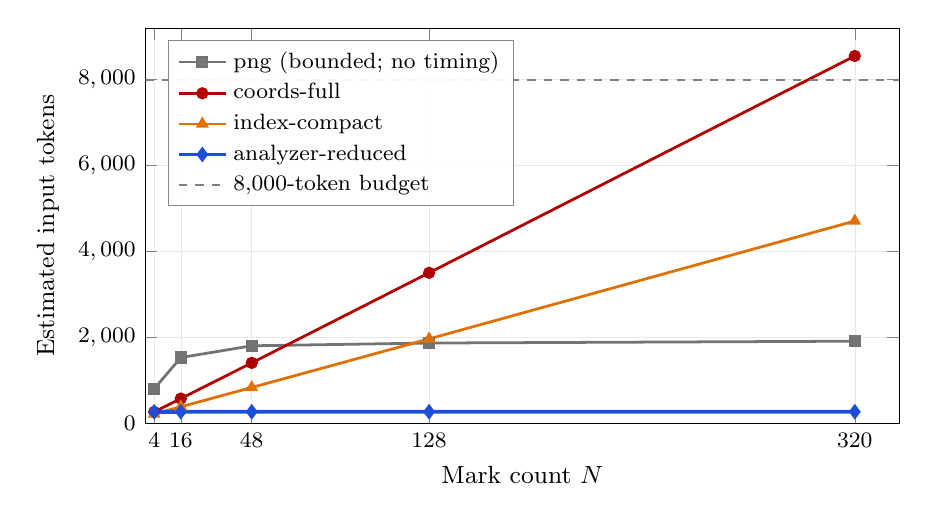
\begin{tikzpicture}
\begin{axis}[
  width=0.92\linewidth, height=6.6cm,
  xlabel={Mark count $N$}, ylabel={Estimated input tokens},
  xmin=0, xmax=340, ymin=0, ymax=9200,
  xtick={4,16,48,128,320},
  scaled y ticks=false, yticklabel style={/pgf/number format/1000 sep={,}},
  legend pos=north west, legend cell align=left,
  legend style={font=\footnotesize, draw=rulegray, fill opacity=0.92, text opacity=1},
  grid=both, grid style={line width=0.2pt, draw=gray!18},
  tick label style={font=\footnotesize}, label style={font=\small},
  every axis plot/.append style={line width=1pt, mark size=1.7pt},
]
\addplot[color=black!55, mark=square*] coordinates {(4,806)(16,1532)(48,1806)(128,1870)(320,1913)};
\addplot[color=red!70!black, mark=*] coordinates {(4,265)(16,577)(48,1408)(128,3506)(320,8554)};
\addplot[color=orange!88!black, mark=triangle*] coordinates {(4,218)(16,386)(48,835)(128,1967)(320,4712)};
\addplot[color=neehblue, mark=diamond*, line width=1.4pt] coordinates {(4,268)(16,269)(48,269)(128,270)(320,270)};
\addplot[dashed, color=gray, line width=0.9pt, mark=none] coordinates {(0,8000)(340,8000)};
\legend{png (bounded; no timing), coords-full, index-compact, analyzer-reduced, 8{,}000-token budget}
\end{axis}
\end{tikzpicture}
\caption{Token cost versus ink density for the temporal task. Both serialized
structured channels answer with 1.00 accuracy at every $N$, but \code{coords-full}
grows roughly linearly and crosses the 8{,}000-token budget near $N{=}320$, while
\code{index-compact} trails it with a smaller slope. The \code{png} raster is
bounded but cannot answer a timing question at all. Only the deterministic
\code{analyzer-reduced} channel is both accurate \emph{and} bounded, sitting flat
at $\approx$270 tokens across the entire range.}
\label{fig:crossover}
\end{figure}

The lesson is architectural. The earlier intuition that ``no current
representation provides bounded cost \emph{and} the temporal signal'' is false: a
task-conditioned local analyzer provides exactly that. The problem that looked
like a case for a learned fixed-size encoder is a token-scaling problem, and a
deterministic reducer solves it exactly, is inspectable and testable, and needs
no model to perform the search.

\subsection{Supporting measurements}
\label{sec:support}

\paragraph{Structured index versus raster on real ink.} On a comparison over real
ink, the two channels cost about the same on a trivial 3-stroke page
($\approx$109 vs 115 tokens), but on a realistic busy page (46 strokes: a
sidebar plus a question) the structured index cost $\approx$190 tokens against
$\approx$1{,}025 for raster-plus-geometry --- \textbf{5.4$\times$ cheaper} ---
because per-stroke SVG geometry and the raster collapse into a marks list with
handwriting summarized as a count~\cite{adr1}. An ASCII ``gestalt'' arm was
\emph{not} a token win (grid whitespace cost more than the index); it is kept
only as a qualitative, model-agnostic fallback for text-only backends.

\paragraph{Delta context and session transport.} Sending only what changed since
the model's last turn, computed from the document's own timestamps, reached 52\%
of a full-resend window's size by turn~3 and $\approx$17\% by turn~10; a
raster-only channel with no delta mechanism showed an outright \emph{capability}
loss on state-tracking (0.00 on an erase-detection task), not merely a cost
increase~\cite{adr3}. A separate study of provider-side stateful session resume
found it a mixed bargain at best: a resumed turn that missed the provider's
prefix cache re-billed the entire prior thread (39k vs 22.5k tokens for a cold
start), and only about half of resumes hit the cache; resumed sessions also
cannot attach images. The resulting ranking across transports was \emph{in-turn
tool loop $>$ cached resume $>$ cold resume $>$ stateless two-shot} --- the
cheapest, most reliable pattern was to give the model more to do \emph{within}
one turn via tool calls, which is the shape the Ink Agent Interface already
takes. These measurements are why Neeh's turns are stateless with
document-derived deltas.

\paragraph{Controlled-pair perception smoke test.} A two-case controlled probe
(identical-raster direction pair, right vs left) confirmed the Experiment-1
mechanism at the level of the full agent stack rather than a bare prompt: the
raster-only policy produced the \emph{same} answer for both twins and therefore
missed one hidden direction (1/2), while the temporal-bootstrap policy
distinguished both (2/2). This is a smoke result, not a statistical accuracy
claim, but it shows the effect survives the perception-policy machinery.

\subsection{Software validation}
\label{sec:software}

The SDK itself is validated by an automated test suite that passes in full.
Table~\ref{tab:tests} inventories the Python tests by area; all
\textbf{243 tests pass} (in $\approx$0.8\,s). Two native suites --- a C++ core
suite and a C-ABI suite --- also pass. Continuous integration runs the Python
suite on 3.10 and 3.12, builds the native core on Linux and macOS, runs the C and
C++ suites, and verifies the installed CMake package.

\begin{table}[t]
\centering
\small
\begin{tabular}{@{}l r l r@{}}
\toprule
\textbf{Area} & \textbf{Tests} & \textbf{Area} & \textbf{Tests} \\
\midrule
Tool surface        & 47 & Assistant demo        & 10 \\
Ink model           & 34 & Text-ink              & 8  \\
Context (v0)        & 23 & PNG rendering         & 6  \\
Canvas              & 23 & Perception eval       & 6  \\
Document            & 18 & Ink Agent Interface   & 6  \\
Agents              & 16 & SVG/ASCII rendering   & 5  \\
Context v1 (ICF)    & 15 & ASCII gestalt         & 5  \\
UIM adapter         & 10 & Timeline              & 4  \\
                    &    & Analyzers             & 4  \\
                    &    & Protocol discovery    & 3  \\
\midrule
\multicolumn{4}{r}{\textbf{Total: 243 Python tests + 2 native suites, all passing}} \\
\bottomrule
\end{tabular}
\caption{Test inventory. The analyzer tests directly assert the
$\S\ref{sec:move1b}$ property in code: \code{latest\_mark} reduces 320 strokes to
one constant-size record ($<$500 serialized bytes), and the observation
workspace stays within its bootstrap budget on the same 320-mark page.}
\label{tab:tests}
\end{table}

\section{Discussion}
\label{sec:discussion}

\subsection{Why not a learned ink encoder}
An early, reasonable plan for Neeh was a two-track program: ship a structured
product now, and separately pursue a native learned ink encoder --- a
stroke/point encoder feeding learned query tokens into a language model, in the
lineage of BLIP-2's Q-Former~\cite{blip2} --- on the theory that raw ink
trajectories carry information a PNG provably cannot. That existence argument is
\emph{correct} but insufficient. It establishes that \emph{some} representation
beyond a PNG carries the signal; it does not establish that a \emph{learned} one
is the right one when plain structured data already exists as an alternative.

The two experiments test the encoder's would-be value proposition directly and
find it absent at the densities tested:
\begin{itemize}[leftmargin=1.4em, itemsep=2pt]
\item \textbf{On the accuracy axis}, the gap an encoder would close does not
  exist: plain coordinate serialization already maximizes accuracy on the
  history axes (\S\ref{sec:move1}), and accuracy does not degrade with density
  (\S\ref{sec:move1b}). A learned encoder cannot beat 1.00.
\item \textbf{On the cost axis}, where serialization genuinely does break (linear
  growth crossing budget), the problem is solved \emph{exactly} by a
  deterministic reducer at constant cost --- with no training data, no inference
  cost, no privacy surface, and no new model artifact to maintain. The reducer is
  also exact, inspectable, and unit-tested, which a learned fixed-size bottleneck
  is not.
\end{itemize}

We are careful about the scope of the second point. A deterministic reducer
dissolves the cost problem only for tasks that \emph{admit} an exact reduction ---
latest-mark is $\arg\max$ over end times, and creation order, dynamics, and
cross-out candidacy are similarly closed-form. For a question with no known exact
reducer, the fallback is structured retrieval plus targeted raster or geometry,
whose cost scales with the \emph{relevant} evidence rather than the whole page but
is not provably constant. This is not a hole in the argument; it is precisely why
gate condition~(1) below requires a real task to fail under analyzers,
\emph{retrieval, targeted paths, and raster together} before the encoder is
reconsidered. The claim is not ``reduction solves every ink question at constant
cost''; it is ``for the mechanical questions a learned encoder was proposed to
absorb, an exact reducer already does so, and for the rest the open question is
answered by the gate, not assumed away.''

The decision, recorded as ADR 0002~\cite{adr2}, is therefore to \emph{not} build
a native ink encoder, Q-Former-style bridge, or ink pretraining pipeline, and to
put engineering effort into broader analyzer coverage instead. Crucially this is
a \emph{reversible} position with an explicit, falsifiable gate. The
learned-encoder question is reopened only if \emph{all} of the following hold:
(1) a valuable real task repeatedly fails under exact analyzers, structured
retrieval, targeted paths, \emph{and} raster evidence; (2) the failure is
representational rather than a recognizer, data, or tooling defect; (3) a learned
prototype beats the \emph{complete} structured baseline on held-out writers and
devices; and (4) the gain justifies training, inference, privacy, and
maintenance cost. Novelty --- and the encoder$\rightarrow$frozen-model reasoning
question genuinely is unoccupied territory in the literature --- is not by itself
product evidence.

\subsection{The safety dimension}
The confabulation finding (\S\ref{sec:move1}, finding 3) deserves emphasis
because it is orthogonal to cost. Its danger is not merely that a raster-only
assistant fabricates, but \emph{where}: exactly on the questions where a
false visual prior makes the fabrication feel grounded, so the unsafe answers are
the convincing-looking ones, indistinguishable from the safe ones without the very
ink history the raster lacks. For an application reasoning about corrections,
revisions, or provenance in a user's notes --- the tasks ink history exists to
support --- that is a correctness-and-trust hazard, not a mere inefficiency, and
supplying structure converts the confident wrong answer into a grounded right
one.

This failure instantiates the documented tendency of vision-language models to
hallucinate rather than abstain~\cite{pope}, but the render-identical design
probes it more cleanly than a standard object-hallucination benchmark. There,
whether an image supports a claim is itself adjudicated by human or model labels,
so the verdict inherits that noise; here, the twins are certified byte-identical
with opposite ground truth, so the information is \emph{provably} absent and any
confident, differentiated answer is necessarily fabricated --- no adjudication in
the loop. Render-identical pairs may thus be a useful general instrument for
studying confident hallucination under provable information absence, beyond ink.

\subsection{Relationship to the strong baseline}
It is worth restating that Neeh's structured path is not a straw man. The
``recognize $\rightarrow$ structured text $\rightarrow$ model'' pipeline embodied
by diagram-as-code systems~\cite{diagramcode} is training-free and strong, and
Neeh's recognizer-plus-index-plus-tools stack is an instance of it, specialized
to ink. Any future case for a learned encoder must beat this baseline, which is
Neeh's own product --- not merely beat a raster.

\section{Threats to Validity}
\label{sec:threats}

We are explicit about what the evidence does and does not support.

\paragraph{Synthetic, controlled ink.} Both headline experiments use synthetic,
generator-constructed ink --- horizontal strokes, rectangles, arrows, and small
squiggles --- not real handwriting or messy diagrams from real devices and
writers. This is a deliberate trade: it is what makes the pixel-identity
certification exact and the raster floor provably chance. It also means the
finding ``accuracy does not degrade with density'' is strong evidence against an
encoder being \emph{necessary}, not proof that one would never help on messier
real ink. Broadening to real handwriting, math, corrections, and dense notes is
the project's next milestone.

\paragraph{Single model and configuration.} All results use one model (GPT-5.5)
at one reasoning effort, through one provider's CLI. Fixing the model is what
isolates the representation effect, but it means we do not characterize how the
floor, the ceiling, or the confabulation behavior vary across model families or
sizes. A weaker model might, for instance, fail to exploit the coordinate stream
that GPT-5.5 uses so cleanly.

\paragraph{Cell sizes.} The render-identical cells are $n=12$ per condition and
the token-budget cells are 6 trials each. These are large enough to make a
0.50-versus-1.00 separation unambiguous (the effect is categorical, not a small
mean shift) but they are not powered for fine-grained accuracy estimates, and we
report them as such.

\paragraph{Forced-choice answers.} The answer schema offered only the two options,
no ``unknown,'' so a model could not formally abstain; the raw $0.50$ floor
reflects a forced guess. This does not weaken the confabulation finding, which
lives in the free-text ``why'' rather than the picked option: forced to choose,
the model still \emph{fabricated} false evidence on direction ($12/12$) instead of
flagging the guess, as it did on order. An explicit abstention option is the
natural next probe, separating ``cannot abstain'' from ``will not.''

\paragraph{Estimated, not billed, tokens.} Token counts are a deterministic
estimate (chars$/4$ plus pixels$/750$), chosen for offline reproducibility, not
provider-billed token counts. The estimate is used identically across conditions,
so the \emph{relative} comparisons and the crossover are robust; the absolute
budget line ($8{,}000$) is illustrative.

\paragraph{Provenance of supporting numbers.} The context-arm, delta-context, and
session-transport figures (\S\ref{sec:support}) are drawn from the project's
internal experiment log (the ADRs) rather than re-run for this paper; they are
reported as supporting context for architectural decisions, with the two
certified, reproducible experiments carrying the primary claims.

\section{Conclusion and Future Work}

Neeh treats digital ink the way modern GUI agents learned to treat interfaces:
structure first, pixels on demand. We built the structured representation that
digital ink lacked --- an immutable ink model, a compact Ink Context Format,
deterministic analyzers, temporal retrieval, a geometric recognizer, and a
bounded agent loop over MCP --- and we measured whether it earns its place. Two
controlled experiments say it does, and say something sharper: the raster-only
baseline is not just lossy but \emph{unsafe}, confabulating answers the pixels
cannot support; and the ambitious alternative of a learned ink encoder is, on
this evidence, unwarranted, because the accuracy gap it would close does not
exist and the cost problem it would address is solved exactly by a deterministic
reducer.

The roadmap follows the boundary of that evidence. \textbf{M1} broadens the
analysis plane (containment, intersection, connectors, grouping) and separates
recognizer claims from exact measurements with confidence and provenance on every
inferred fact. \textbf{M2} adds an append-only document event log so that
destructive-history claims (\code{history\_complete}) become honest and
erased/replaced ink can be replayed. \textbf{M3} --- the decisive one for the
encoder question, and the milestone that would lift this paper's central
limitation --- \emph{seeks to establish} grounding on \emph{real} ink from real
devices and writers (all evidence here is synthetic), comparing raster-only,
raster+geometry, index-only, active-index,
marked-index, and analyzer-first policies with the model fixed, and measuring
target accuracy, abstention, false explanations, retrieval calls, context,
pixels, latency, and human acceptance under adversarial contamination controls.
\textbf{M4} and \textbf{M5} stabilize and publish the agent protocols and prepare
a first externally consumable release. The learned-encoder gate stays open,
empirical, and falsifiable: if a valuable real task defeats the complete
structured baseline for representational reasons, the question reopens --- and
until then, the structured baseline is the product.

\section*{Reproducibility}

The two headline experiments are driven by \code{research/move1\_render\_identical\_pairs.py}
and \code{research/move1b\_token\_budget.py}. Both support a \code{--dry-run} mode
that certifies pixel identity and prices every prompt with no model calls, and a
live \code{--agent codex} sweep pinned to GPT-5.5 at high reasoning effort. Raw
per-trial results are archived as JSON under \code{research/}. The SDK and its
243-test suite install from a checkout with \code{python -m pip install -e ".[dev]"}
and run with \code{python -m pytest -q}; the native suites build with CMake and
run under \code{ctest}. Neeh is open source under the Apache License 2.0 at
\url{https://github.com/kunwarpadda/Neeh-SDK}~\cite{neeh}; see \code{CITATION.cff}
for citation metadata.

\begin{thebibliography}{99}
\footnotesize
\setlength{\itemsep}{0pt}
\setlength{\parskip}{0pt}

\bibitem{fadeeva2024}
A.~Fadeeva et al.
\newblock Representing Online Handwriting for Recognition in Large Vision-Language Models.
\newblock arXiv:2402.15307, 2024.

\bibitem{cololhtr}
Y.~Liu et al.
\newblock Col-OLHTR: A Collaborative Multimodal Framework for Online Handwritten Text Recognition.
\newblock arXiv:2502.06100, 2025.

\bibitem{lodh2025}
S.~Lodh et al.
\newblock A Transformer-Based Handwriting Recognition System Jointly Using Online and Offline Features.
\newblock Asian Conf.\ on Pattern Recognition (ACPR), arXiv:2506.20255, 2025.

\bibitem{scribetokens}
Wang.
\newblock ScribeTokens: Fixed-Vocabulary Tokenization of Digital Ink.
\newblock arXiv:2603.02805, 2026.

\bibitem{inksight}
InkSight.
\newblock Offline-to-Online Handwriting Conversion by Teaching Vision-Language Models to Read and Write.
\newblock arXiv:2402.05804, 2024.

\bibitem{flamingo}
J.-B.~Alayrac et al.
\newblock Flamingo: a Visual Language Model for Few-Shot Learning.
\newblock arXiv:2204.14198, 2022.

\bibitem{blip2}
J.~Li, D.~Li, S.~Savarese, and S.~Hoi.
\newblock BLIP-2: Bootstrapping Language-Image Pre-training with Frozen Image Encoders and Large Language Models.
\newblock arXiv:2301.12597, 2023.

\bibitem{llava}
H.~Liu, C.~Li, Q.~Wu, and Y.~J.~Lee.
\newblock Visual Instruction Tuning (LLaVA).
\newblock arXiv:2304.08485, 2023.

\bibitem{pope}
Y.~Li, Y.~Du, K.~Zhou, J.~Wang, W.~X.~Zhao, and J.-R.~Wen.
\newblock Evaluating Object Hallucination in Large Vision-Language Models (POPE).
\newblock Proc.\ EMNLP, 2023.

\bibitem{setofmark}
J.~Yang et al.
\newblock Set-of-Mark Prompting Unleashes Extraordinary Visual Grounding in GPT-4V.
\newblock arXiv:2310.11441, 2023.

\bibitem{omniparser}
Y.~Lu et al.
\newblock OmniParser for Pure Vision-Based GUI Agent.
\newblock arXiv:2408.00203, 2024.

\bibitem{memgpt}
C.~Packer et al.
\newblock MemGPT: Towards LLMs as Operating Systems.
\newblock arXiv:2310.08560, 2023.

\bibitem{diagramcode}
Draw-with-Thought; SketchAgent; CoMT.
\newblock The diagram-reasoning-as-code line of work (structured/XML program recovery for figure understanding), 2025--2026.

\bibitem{mcp}
Anthropic.
\newblock Model Context Protocol (MCP) specification.
\newblock \url{https://modelcontextprotocol.io}, 2024.

\bibitem{uim}
Wacom.
\newblock Universal Ink Model (UIM) / Ink Markup and Interchange, WILL technology.
\newblock Open ink interchange specification.

\bibitem{inkml}
Y.-M.~Chee, M.~Froumentin, and S.~M.~Watt (eds.).
\newblock Ink Markup Language (InkML).
\newblock W3C Recommendation, 2011.

\bibitem{adr1}
Neeh SDK.
\newblock ADR 0001: Structured index is the primary model-facing channel; raster is fetched on demand.
\newblock In \code{docs/adr/}, 2026.

\bibitem{adr2}
Neeh SDK.
\newblock ADR 0002: Deterministic local analyzers, not a learned ink encoder, for bounded temporal/geometric evidence.
\newblock In \code{docs/adr/}, 2026.

\bibitem{adr3}
Neeh SDK.
\newblock ADR 0003: Stateless-per-turn model sessions with document-derived delta context.
\newblock In \code{docs/adr/}, 2026.

\bibitem{neeh}
K.~S.~Padda.
\newblock Neeh SDK: a structured digital-ink SDK for notebook, whiteboard, and handwriting applications.
\newblock Software, Apache-2.0, version 0.2.0, 2026. See \code{CITATION.cff}.

\end{thebibliography}

\end{document}
